%!TEX root = ../main.tex

\subsection{\cite{buhren_one_2021} - One Glitch to Rule Them All: Fault Injection Attacks Against AMD's Secure Encrypted Virtualization} 

\textbf{One Glitch to Rule Them All: Fault Injection Attacks Against AMD's Secure Encrypted Virtualization }

\subsubsection*{Abstract \cite{buhren_one_2021}}
“AMD Secure Encrypted Virtualization (SEV) offers protection mechanisms for virtual machines in untrusted environments through memory and register encryption. To separate security-sensitive operations from software executing on the main x86 cores, SEV leverages the AMD Secure Processor (AMD-SP). This paper introduces a new approach to attack SEV-protected virtual machines (VMs) by targeting the AMD-SP. We present a voltage glitching attack that allows an attacker to execute custom payloads on the AMD-SPs of all microarchitectures that support SEV currently on the market (Zen 1, Zen 2, and Zen 3). The presented methods allow us to deploy a custom SEV firmware on the AMD-SP, which enables an adversary to decrypt a VM's memory. Furthermore, using our approach, we can extract endorsement keys of SEV-enabled CPUs, which allows us to fake attestation reports or to pose as a valid target for VM migration without requiring physical access to the target host. Moreover, we reverse-engineered the Versioned Chip Endorsement Key (VCEK) mechanism introduced with SEV Secure Nested Paging (SEV-SNP). The VCEK binds the endorsement keys to the firmware version of TCB components relevant for SEV. Building on the ability to extract the endorsement keys, we show how to derive valid VCEKs for arbitrary firmware versions. With our findings, we prove that SEV cannot adequately protect confidential data in cloud environments from insider attackers, such as rogue administrators, on currently available CPUs.”

\subsubsection*{Conclusion  \cite{buhren_one_2021}}
“The attacks presented in this paper highlight SEV’s insufficient protection against physical attacks. Despite its crucial role for SEV’s security properties, the AMD-SP can be tricked into executing attacker-controlled code. The hardware setup to mount the presented glitching attack is cheap and readily available. Building on this setup, we presented how an adversary with physical access to the target host can implant a custom SEV firmware that decrypts a VM’s memory using SEV’s debug API calls.

Furthermore, we showed that the glitching attack enables the extraction of endorsement keys. The endorsement keys play a central role in the remote attestation mechanism of SEV and can be used to mount software-only attacks. Even an attacker without physical access to the target host can use extracted endorsement keys to attack SEV-protected VMs. By faking attestation reports, an attacker can pose as a valid target for VM migration to gain access to a VM’s data. The severity of the presented software-only attacks is amplified by the fact that an attacker can perform the key extraction on an AMD CPU unrelated to the CPU hosting the targeted VM, i.e., on an AMD Epyc CPU bought by the attacker for the sole purpose of extracting an endorsement key.

Our analysis revealed that the TCB versioning scheme introduced with SEV-SNP does not protect against the presented attacks. Based on our results, we conclude that SEV cannot adequately protect confidential data in cloud environments from insider attackers, such as rogue administrators. The presented attacks do not rely on firmware issues and can not be easily mitigated. Hence, we proposed mitigations for future AMD Epyc CPUs. Nevertheless, to the best of our knowledge, all AMD Epyc CPUs of the Zen 1, Zen 2 and Zen 3 microarchitectures are susceptible to the presented attacks. ”


\url{https://github.com/PSPReverse/amd-sp-glitch }

\begin{figure}[!ht]
    \centering
    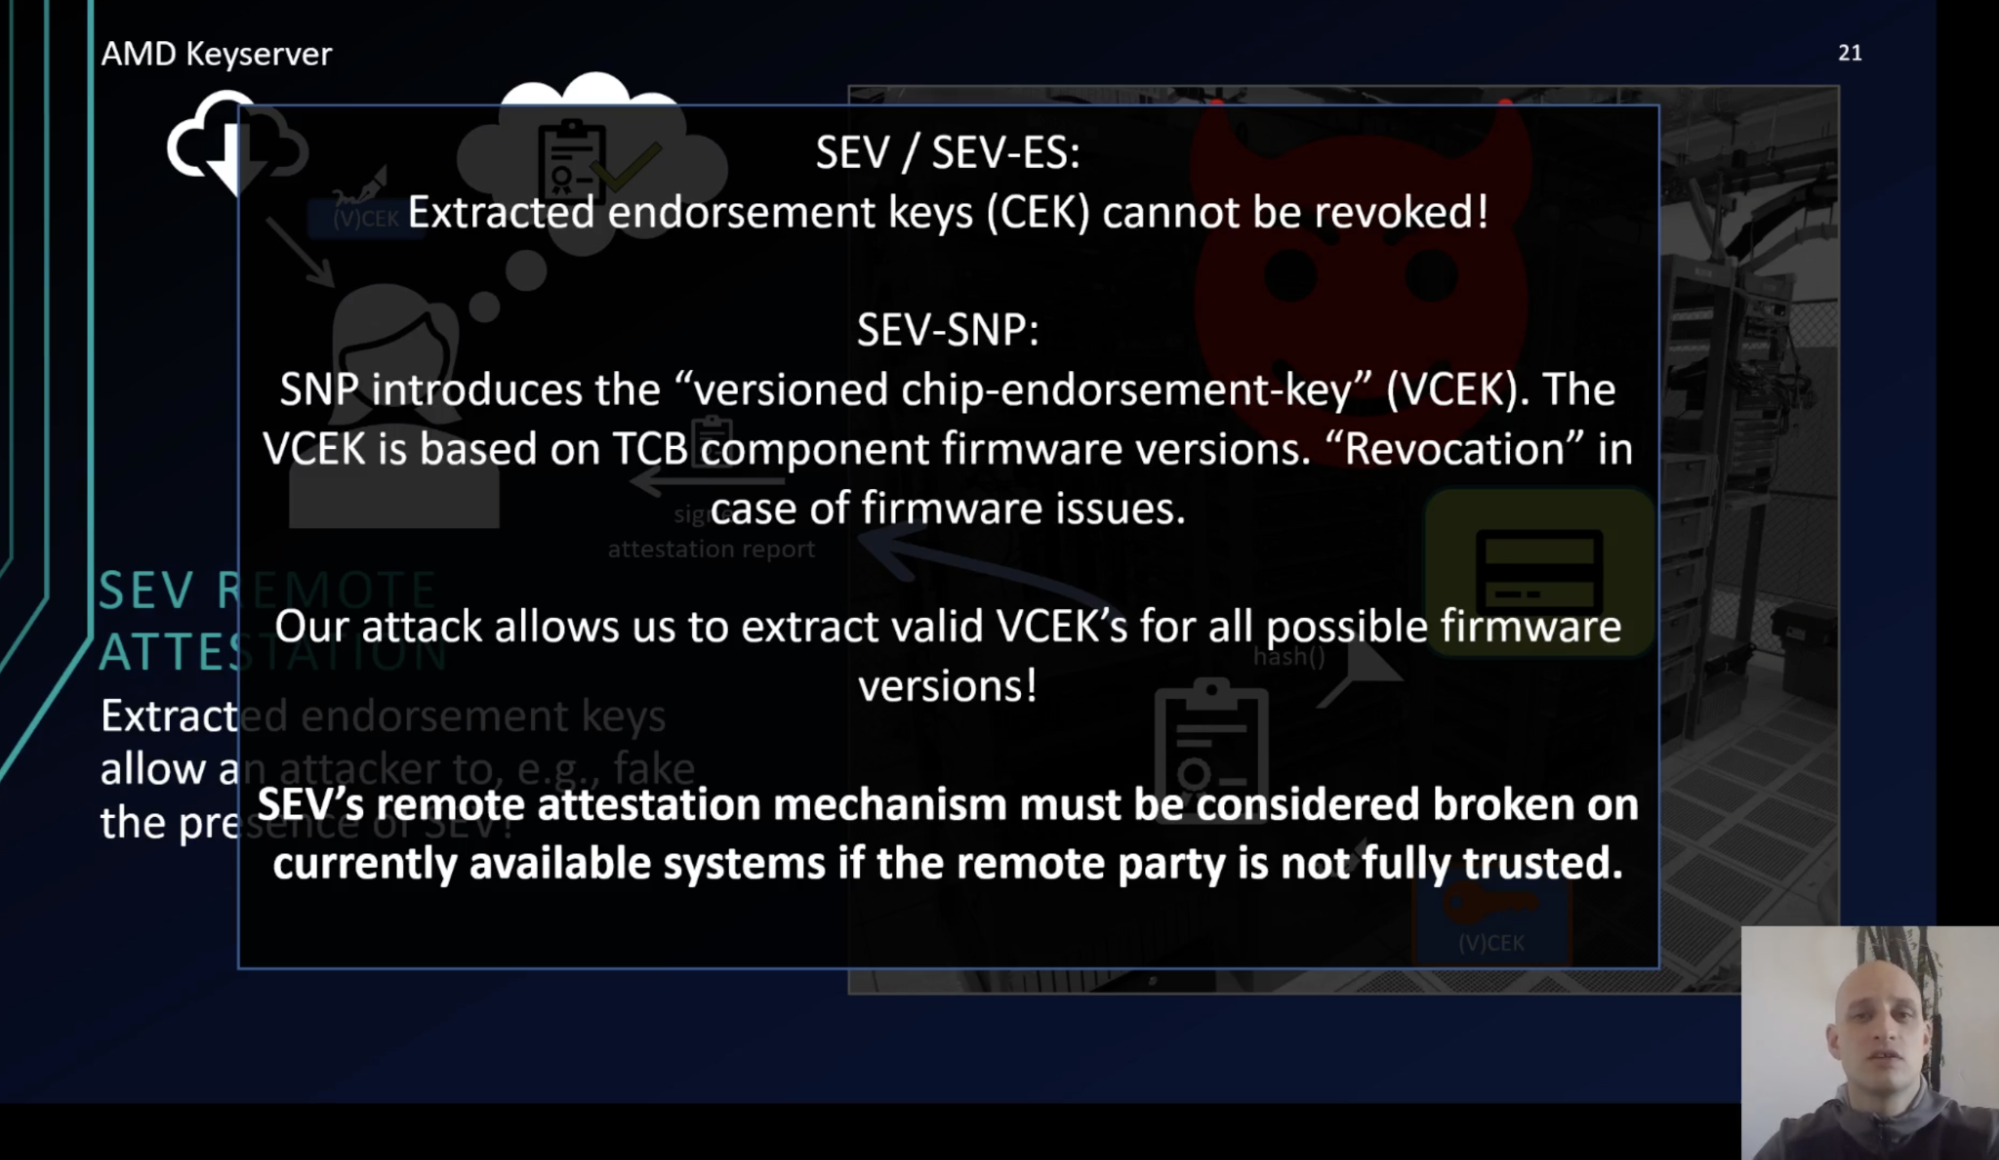
\includegraphics[width=0.6\linewidth]{buhren-1}
    \caption{Image from \cite{buhren_one_2021}}
    \label{fig:buhren-1}
\end{figure}

\begin{figure}[!ht]
    \centering
    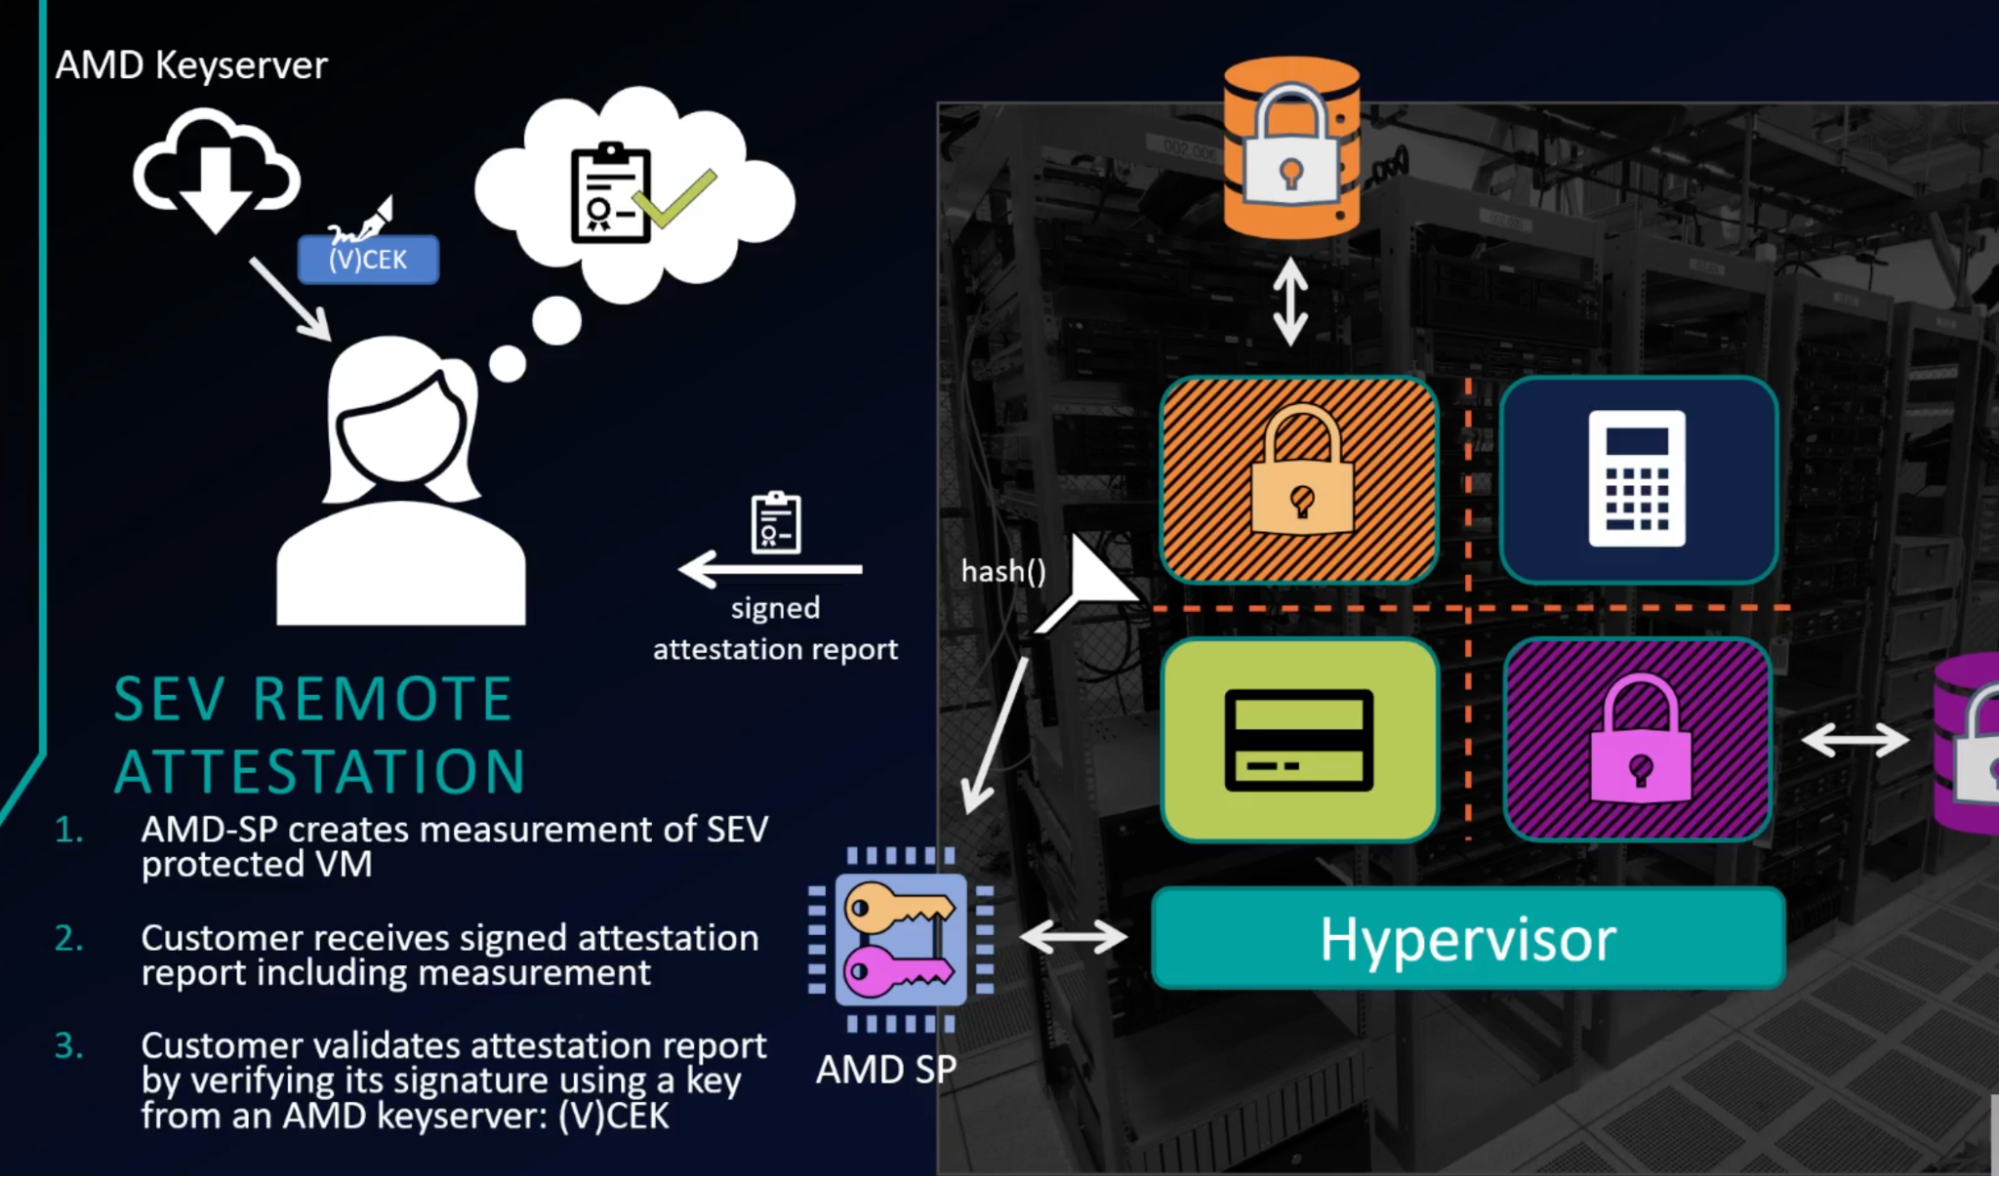
\includegraphics[width=0.6\linewidth]{buhren-2}
    \caption{Image from \cite{buhren_one_2021}}
    \label{fig:buhren-2}
\end{figure}
\begin{figure}[!ht]
    \centering
    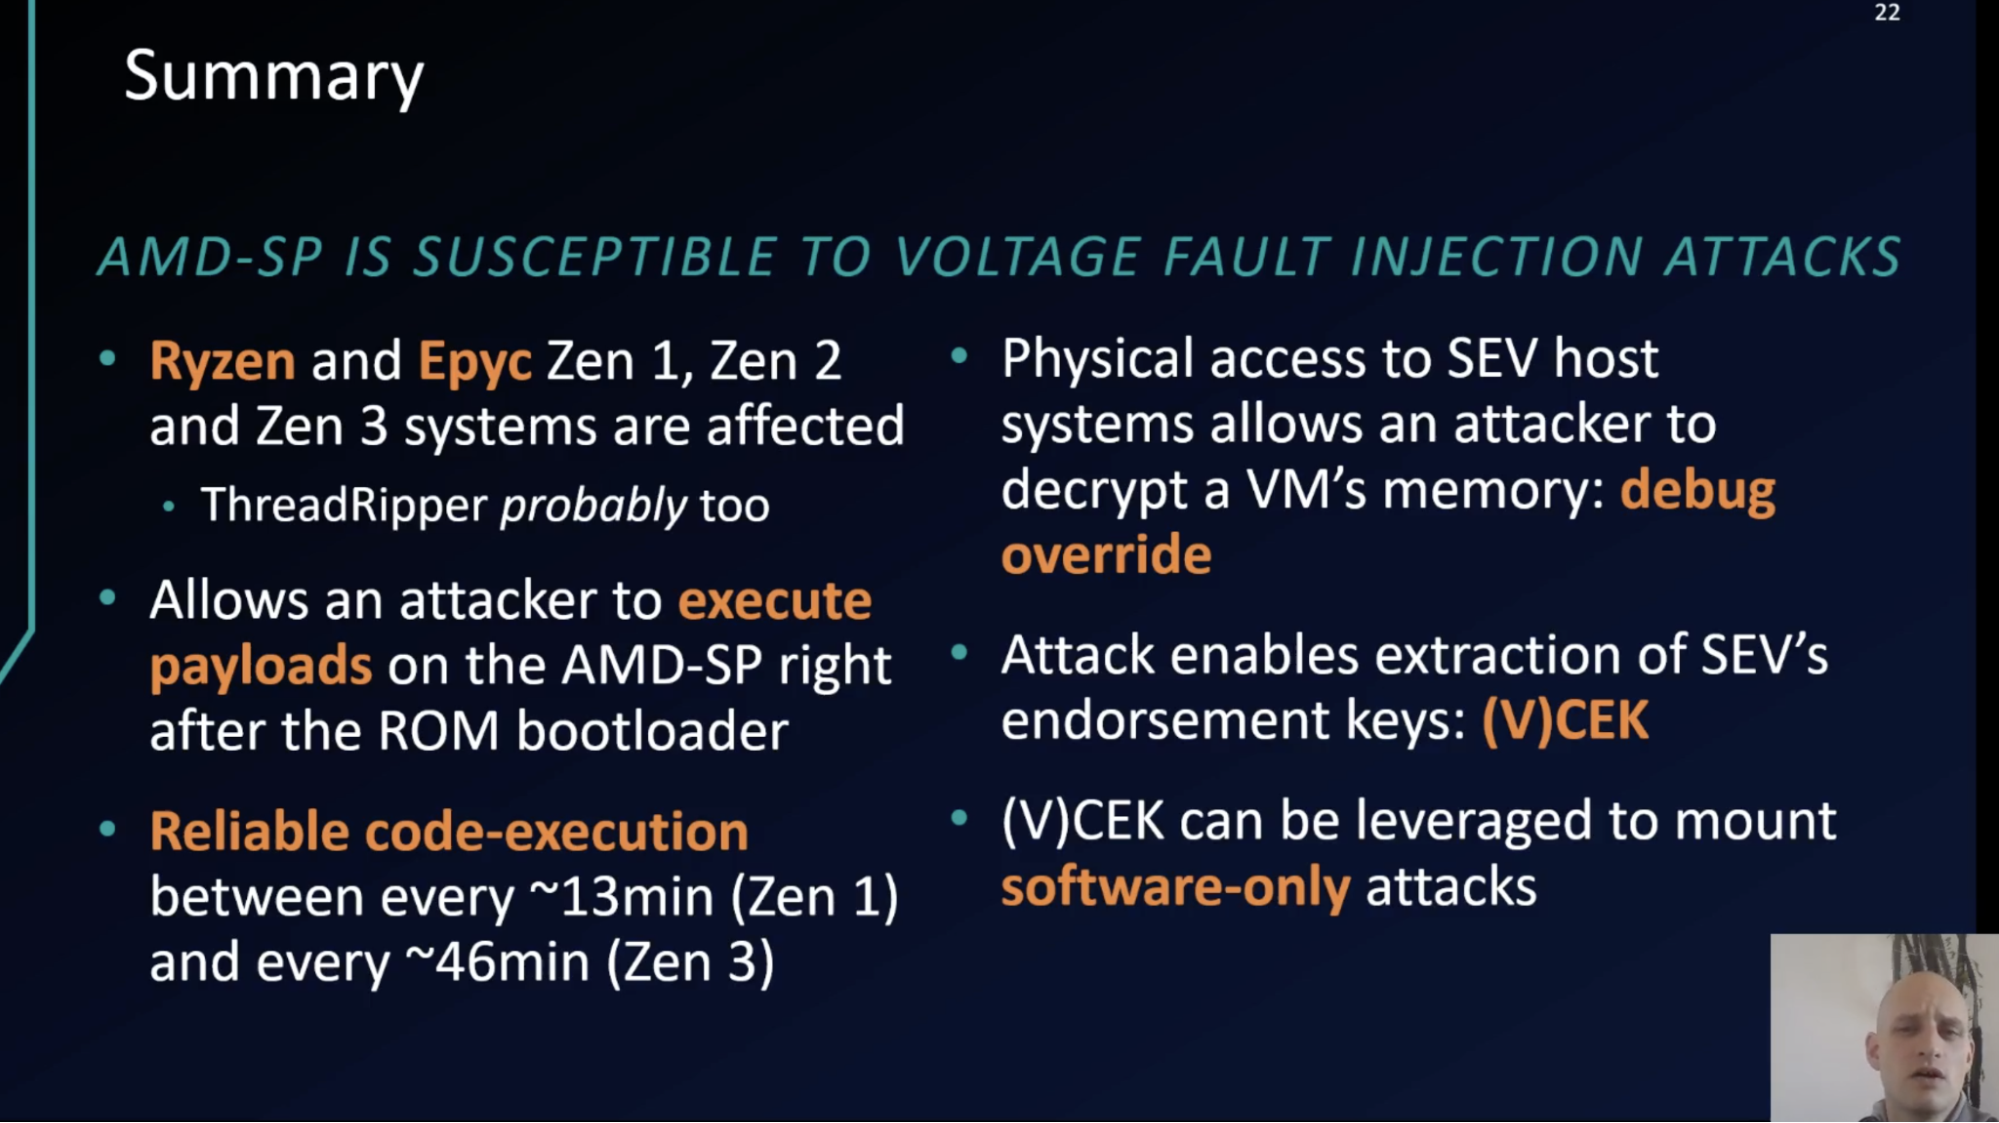
\includegraphics[width=0.6\linewidth]{buhren-3}
    \caption{Image from \cite{buhren_one_2021}}
    \label{fig:buhren-3}
\end{figure}
